\documentclass[xcolor=table]{beamer}

% \rowcolors{1}{gray!30}{gray!10}

\usetheme{Boadilla}
\usecolortheme{dolphin}
\useoutertheme[subsection=false]{smoothbars}

\setbeamercolor{frametitle}{fg = black, bg = white} 
\setbeamercolor{palette primary}{use=structure,fg=white,bg=structure.fg!60!white}
\setbeamercolor{palette secondary}{use=structure,fg=white,bg=structure.fg!90!white}
\setbeamercolor{palette tertiary}{use=structure,fg=white,bg=structure.fg!120!white}
\setbeamercolor{palette quaternary}{use=structure,fg=black,bg=white} %Top bar

\setbeamertemplate{enumerate subitem}[circle]%
\renewcommand{\insertsubenumlabel}{\alph{enumii}}

\usepackage{amsmath}
\usepackage{xcolor}
\usepackage{booktabs}
\usepackage[utf8]{inputenc}
\usepackage{hyperref}
\usepackage[table]{xcolor}
\definecolor{lightgray}{gray}{0.9}

\hypersetup{
    colorlinks,
    citecolor=blue,
    linkcolor=blue
}

\footnotesize \let\small\footnotesize

\author{Jonathan P. Latner, PhD}
\title{A/B test results}
\date{\today}

\beamertemplatenavigationsymbolsempty 
\setbeamerfont{page number in head/foot}{size=\tiny}
\setbeamertemplate{footline}[frame number]
\setbeamertemplate{caption}[numbered]
\setbeamertemplate{section in toc}[sections numbered]

\begin{document}

\frame{\frametitle{ }
\titlepage
\thispagestyle{empty}
}

\frame{\frametitle{Overview}
\begin{itemize}
    \item A/B test conducted during the month January, 2019
    \item Sample size 743 ($\approxeq$ 24 individuals per day)
    \item Results suggest no effect of treatment on outcomes
\end{itemize}
}

\frame{\frametitle{A/B test sample}
Size = 743 (even split by treatment)

\begin{figure}
    \caption{Treatment}
    \resizebox{\textwidth}{!}{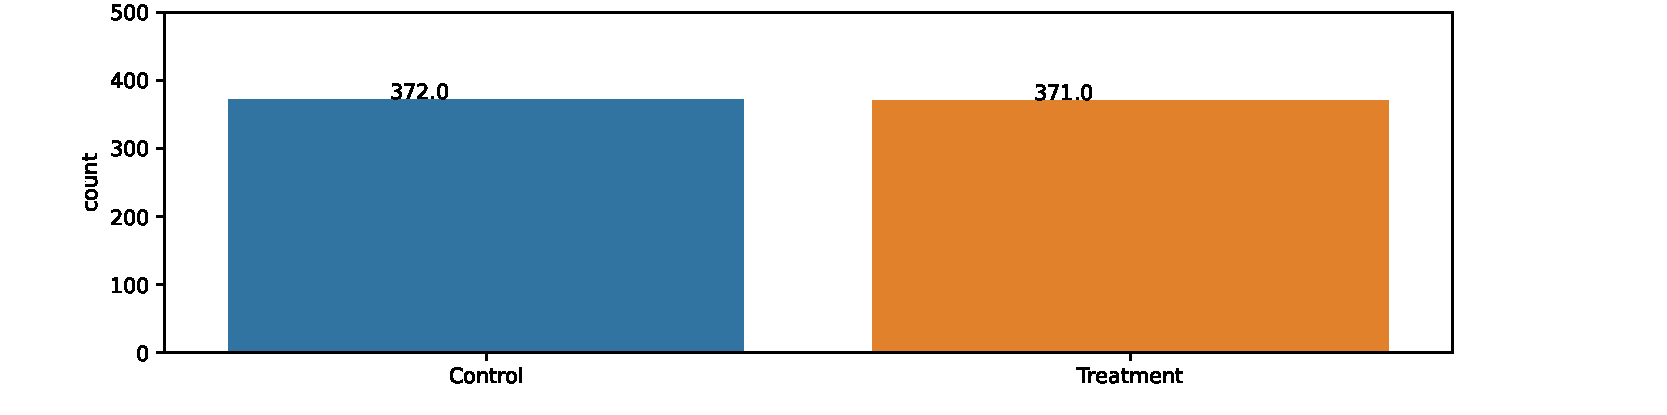
\includegraphics{../graphs/plot_treatment.pdf}}
    \label{plot_treatment}
\end{figure}
}

\frame{\frametitle{Time period}
One month, January 2019

$\approxeq$ 12 individuals per day
\begin{figure}
    \caption{Treatment by date}
    \resizebox{\textwidth}{!}{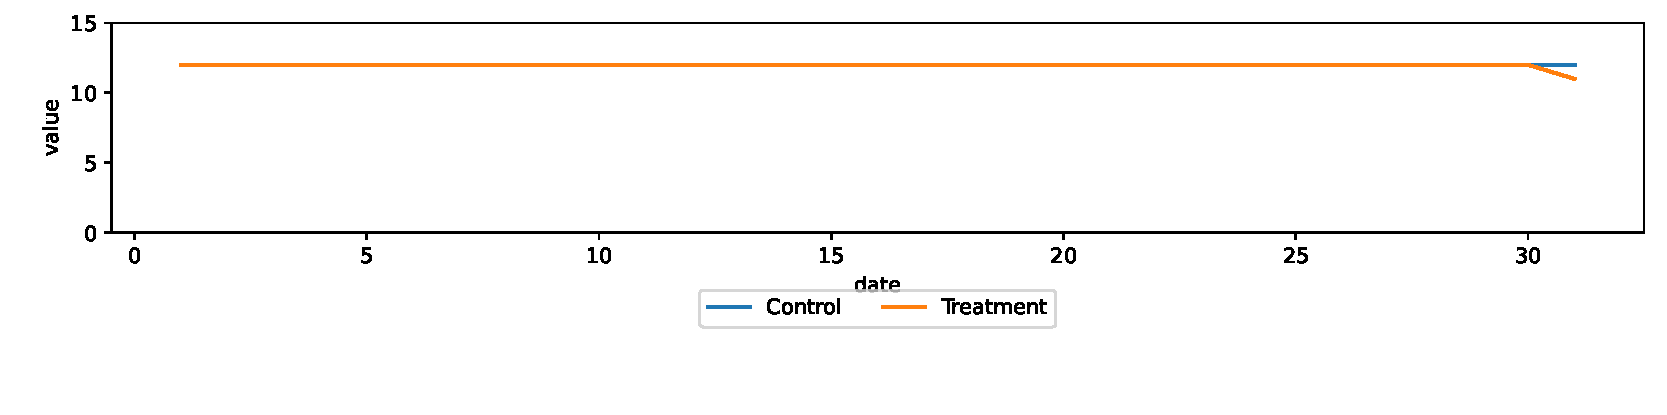
\includegraphics{../graphs/plot_treatment_date.pdf}}
    \label{plot_treatment_date}
\end{figure}
}

\frame{\frametitle{Descriptives - numerical variable}
No difference between treatment and control

\begin{figure}
    \caption{Numerical variables by treatment}
    \resizebox{\textwidth}{!}{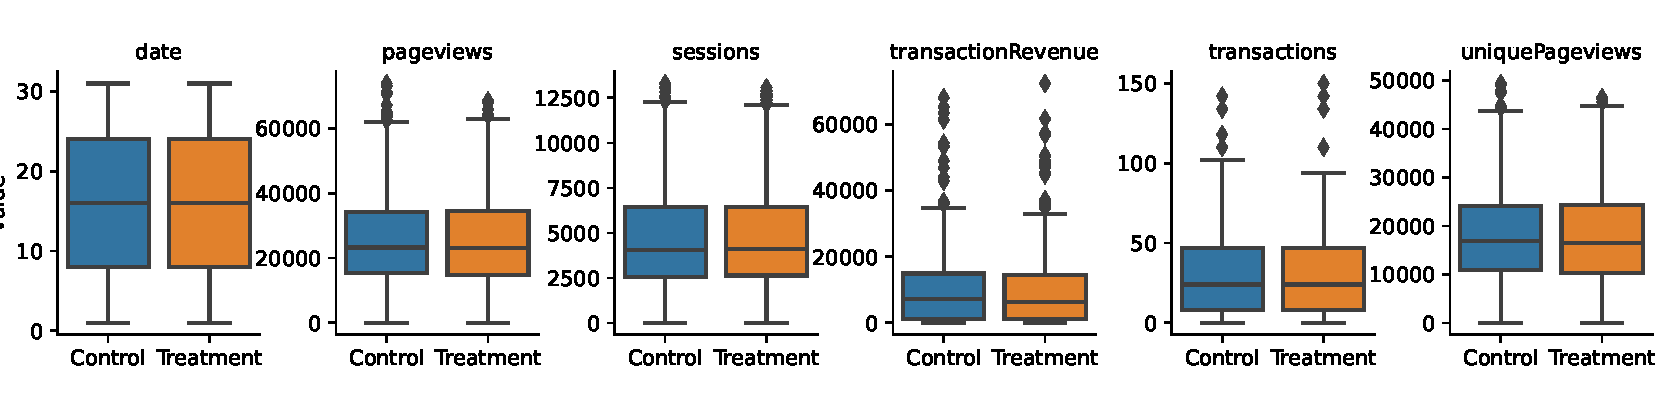
\includegraphics{../graphs/plot_numerical.pdf}}
    \label{plot_numerical}
\end{figure}
}

\frame{\frametitle{Descriptives - categorical variable}
No difference between treatment and control

\begin{figure}
    \caption{Categorical variable (device) by treatment}
    \resizebox{\textwidth}{!}{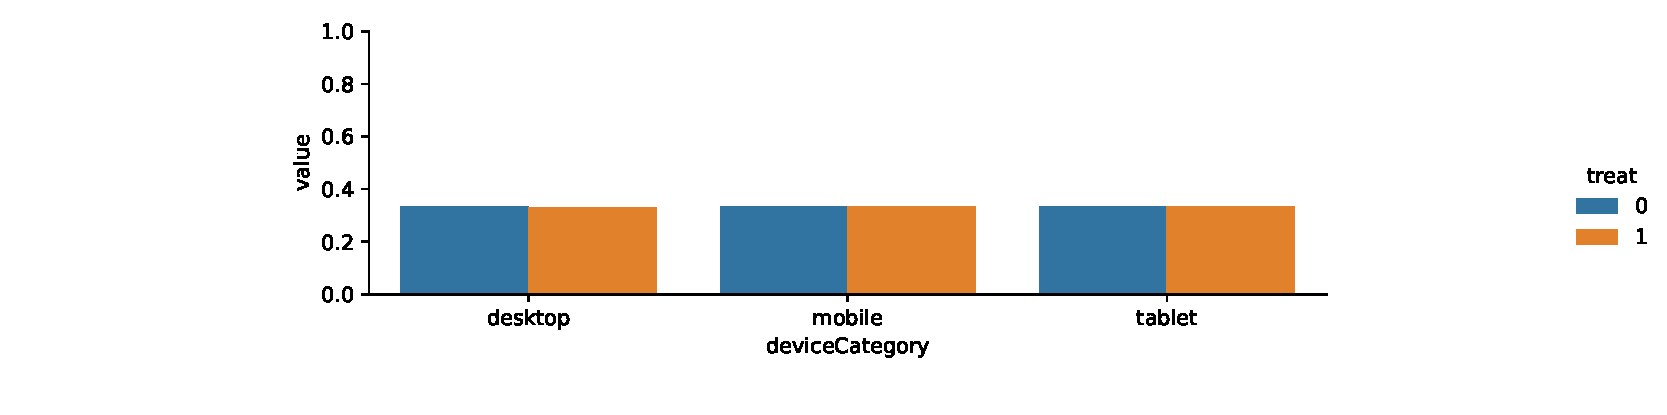
\includegraphics{../graphs/plot_categorical.pdf}}
    \label{plot_category}
\end{figure}
}

\frame{\frametitle{Descriptives - crosstab numerical and control}
Difference between devices
\begin{itemize}
    \item Mobile has higher pageviews, uniqeviews, and sessions
    \item Tablet has lower revenues and transactions
    \item Desktop has slightly higher revenues than mobiles
\end{itemize}

But, no difference between treatment and control

\begin{figure}
    \caption{Numerical variables by device and treatment}
    \resizebox{\textwidth}{!}{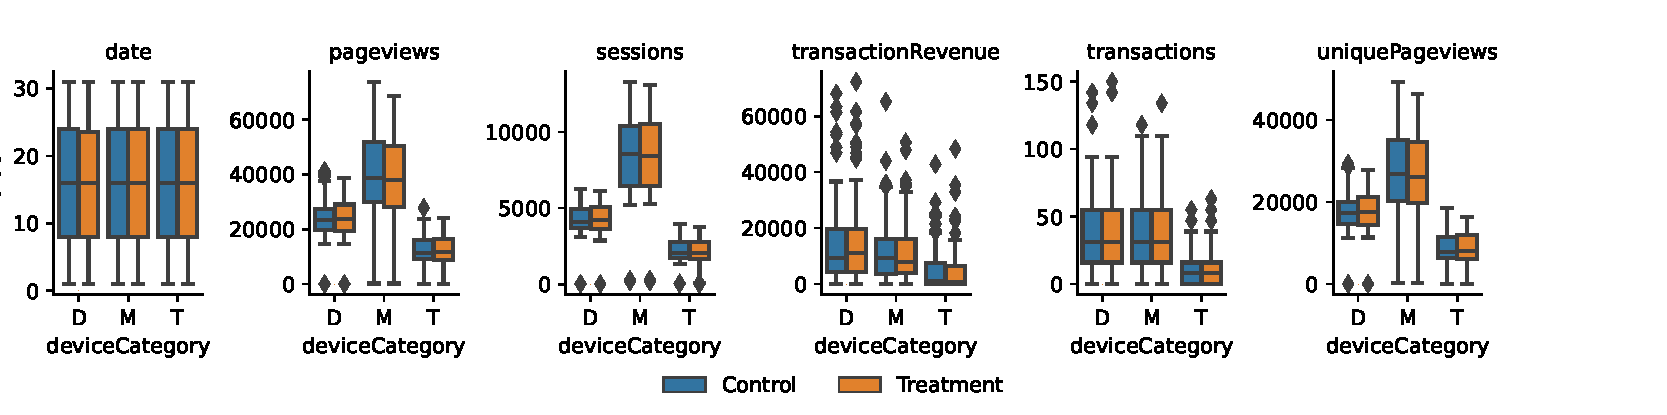
\includegraphics{../graphs/plot_interaction_twoway.pdf}}
    \label{plot_interaction_twoway}
\end{figure}
}

\frame{\frametitle{What about a new variable?}
Avg. revenue per transaction = revenue/transaction

Among tablet users, treatment appears to reduce outliers, but not average

\begin{figure}
    \caption{Average revenue per transaction by device and treatment}
    \resizebox{\textwidth}{!}{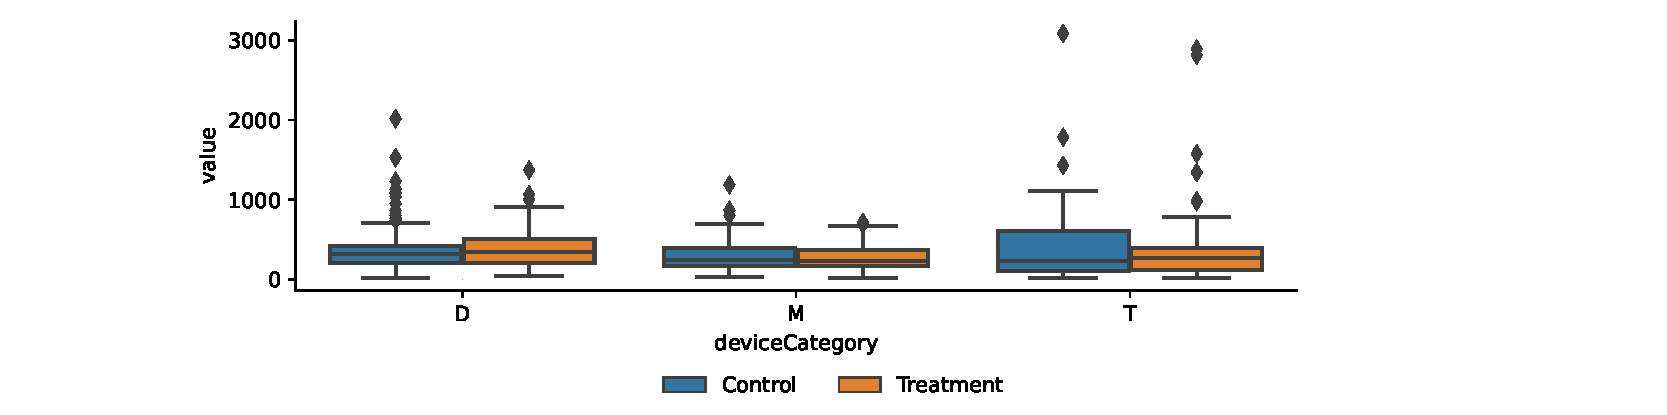
\includegraphics{../graphs/plot_new.pdf}}
    \label{plot_new}
\end{figure}
}


\frame{\frametitle{Time trends}

Variables are declining over time by device category

No difference trends over time by treatment

\begin{figure}
    \caption{Numerical variables over time by device and treatment}
    \resizebox{\textwidth}{!}{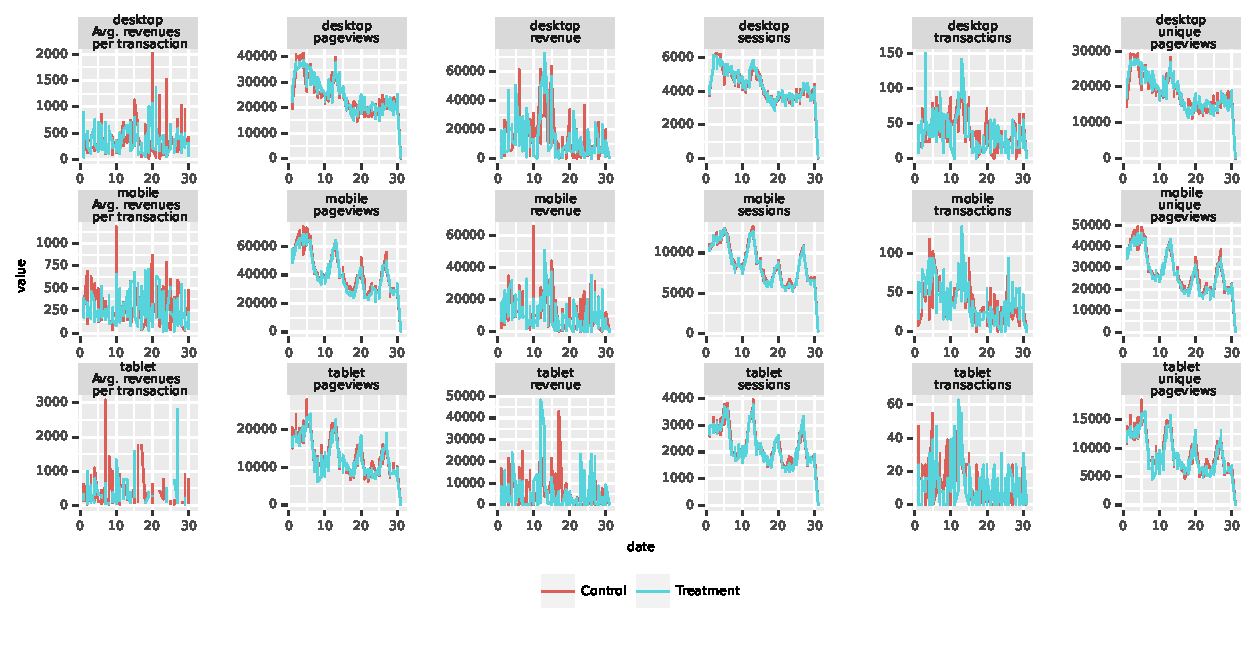
\includegraphics{../graphs/plot_time_trend.pdf}}
    \label{plot_time_trend}
\end{figure}
}

% \frame{\frametitle{Pystout} 

%     \begin{table}[!h]
%     \caption{Parameter estimates of effect of device and treatment on outcomes}
%         \begin{center}
%             \resizebox{.75\textwidth}{!}{\input{../tables/test_table.tex}}
%             \label{test_table.tex}
%         \end{center}
%     \end{table}
% }

\frame{\frametitle{Regressions} 
Model 0 only has main effect of device category and treatment

Model 1 adds an interaction between device category and treatment

Regression models confirm descriptive statistics

There is a main effect of Device category, but no effect of treatment 


    \begin{table}[!h]
    \caption{Parameter estimates of effect of device and treatment on outcomes}
        \begin{center}
            \resizebox{\textwidth}{!}{{
\def\sym#1{\ifmmode^{#1}\else\(^{#1}\)\fi}
\begin{tabular}{@{\extracolsep{2pt}}l*{12}{c}@{}}
\hline\hline
& \multicolumn{2}{c}{Sessions} & \multicolumn{2}{c}{Pageviews} & \multicolumn{2}{c}{Unique views} & \multicolumn{2}{c}{Transactions} & \multicolumn{2}{c}{Revenue} & \multicolumn{2}{c}{Avg. Rev per Trns} \\
\cline{2-3}
\cline{4-5}
\cline{6-7}
\cline{8-9}
\cline{10-11}
\cline{12-13}
 & 0 & 1 & 0 & 1 & 0 & 1 & 0 & 1 & 0 & 1 & 0 & 1 \\
\hline
deviceCategory[T.mobile] & 4199.86\sym{**} & 4292.09\sym{**} & 15819.55\sym{**} & 16562.90\sym{**} & 9521.38\sym{**} & 10014.29\sym{**} & 1.53 & 1.53 & -3324.78\sym{**} & -2573.68\sym{+} & -89.01\sym{**} & -69.71\sym{+} \\
 & (157.37) & (222.58) & (919.92) & (1300.84) & (625.99) & (885.21) & (2.09) & (2.95) & (1012.79) & (1432.07) & (29.28) & (41.51) \\
deviceCategory[T.tablet] & -2032.85\sym{**} & -1984.10\sym{**} & -11734.81\sym{**} & -11357.18\sym{**} & -9163.58\sym{**} & -8876.89\sym{**} & -25.37\sym{**} & -24.65\sym{**} & -9641.13\sym{**} & -8884.33\sym{**} & 32.53 & 52.02 \\
 & (157.37) & (222.58) & (919.92) & (1300.84) & (625.99) & (885.21) & (2.09) & (2.95) & (1012.79) & (1432.07) & (32.29) & (45.01) \\
treat[T.Treatment] & -14.66 & 79.70 & -275.55 & 474.80 & -101.01 & 420.84 & 0.28 & 0.76 & -36.62 & 972.73 & -15.13 & 9.49 \\
 & (128.45) & (223.03) & (750.86) & (1303.48) & (510.95) & (887.01) & (1.70) & (2.96) & (826.66) & (1434.98) & (25.20) & (41.60) \\
deviceCategory[T.mobile]:treat[T.Treatment] &  & -184.83 &  & -1489.73 &  & -987.93 &  & 0.00 &  & -1506.28 &  & -38.45 \\
 &  & (315.09) &  & (1841.53) &  & (1253.15) &  & (4.18) &  & (2027.31) &  & (58.64) \\
deviceCategory[T.tablet]:treat[T.Treatment] &  & -97.86 &  & -758.30 &  & -575.51 &  & -1.46 &  & -1517.69 &  & -39.68 \\
 &  & (315.09) &  & (1841.53) &  & (1253.15) &  & (4.18) &  & (2027.31) &  & (64.70) \\
Intercept & 4239.36\sym{**} & 4192.37\sym{**} & 24507.43\sym{**} & 24133.77\sym{**} & 18047.76\sym{**} & 17787.89\sym{**} & 37.21\sym{**} & 36.97\sym{**} & 14528.87\sym{**} & 14026.24\sym{**} & 381.25\sym{**} & 368.83\sym{**} \\
 & (128.45) & (157.39) & (750.86) & (919.83) & (510.95) & (625.94) & (1.70) & (2.09) & (826.66) & (1012.63) & (24.35) & (29.54) \\

\hline
Obs & 743 & 743 & 743 & 743 & 743 & 743 & 743 & 743 & 743 & 743 & 631 & 631 \\
Adj. R\sym{2} & 0.69 & 0.69 & 0.55 & 0.55 & 0.55 & 0.54 & 0.22 & 0.22 & 0.11 & 0.11 & 0.02 & 0.02 \\
\hline\hline
\end{tabular}
}}
            \label{table_regression.tex}
        \end{center}
    \end{table}
}

\frame{\frametitle{Regressions} 
Model 2 adds main effect of date

Model 3 adds an interaction with date

Regression models confirm descriptive statistics (declining trends)

Tablets trends are still negative: interaction with date $<$ main effect

    \begin{table}[!h]
    \caption{Parameter estimates of effect of device and treatment on outcomes}
        \begin{center}
            \resizebox{\textwidth}{!}{{
\def\sym#1{\ifmmode^{#1}\else\(^{#1}\)\fi}
\begin{tabular}{@{\extracolsep{2pt}}l*{12}{c}@{}}
\hline\hline
& \multicolumn{2}{c}{Sessions} & \multicolumn{2}{c}{Pageviews} & \multicolumn{2}{c}{Unique views} & \multicolumn{2}{c}{Transactions} & \multicolumn{2}{c}{Revenue} & \multicolumn{2}{c}{Avg. Rev per Trns} \\
\cline{2-3}
\cline{4-5}
\cline{6-7}
\cline{8-9}
\cline{10-11}
\cline{12-13}
 & 2 & 3 & 2 & 3 & 2 & 3 & 2 & 3 & 2 & 3 & 2 & 3 \\
\hline
deviceCategory[T.mobile] & 4207.06\sym{**} & 6426.77\sym{**} & 15865.33\sym{**} & 26364.37\sym{**} & 9552.70\sym{**} & 16280.17\sym{**} & 1.60 & 4.92 & -3304.55\sym{**} & -4210.15\sym{+} & -89.01\sym{**} & -54.36 \\
 & (125.31) & (254.32) & (692.41) & (1436.44) & (469.26) & (977.97) & (1.93) & (4.35) & (977.39) & (2225.91) & (29.31) & (66.46) \\
deviceCategory[T.tablet] & -2025.65\sym{**} & -2504.97\sym{**} & -11689.03\sym{**} & -15328.50\sym{**} & -9132.27\sym{**} & -11817.11\sym{**} & -25.31\sym{**} & -36.17\sym{**} & -9620.90\sym{**} & -13531.43\sym{**} & 32.60 & 46.66 \\
 & (125.31) & (254.32) & (692.41) & (1436.44) & (469.26) & (977.97) & (1.93) & (4.35) & (977.39) & (2225.91) & (32.35) & (70.90) \\
treat[T.Treatment] & -19.46 & 66.06 & -306.07 & 463.26 & -121.88 & 392.07 & 0.24 & -0.36 & -50.11 & 951.94 & -15.14 & 0.46 \\
 & (102.28) & (226.34) & (565.16) & (1278.38) & (383.02) & (870.36) & (1.57) & (3.87) & (797.76) & (1980.99) & (25.22) & (61.07) \\
date & -118.36\sym{**} & -84.71\sym{**} & -752.85\sym{**} & -628.79\sym{**} & -514.99\sym{**} & -444.58\sym{**} & -1.00\sym{**} & -1.20\sym{**} & -332.67\sym{**} & -462.84\sym{**} & 0.08 & 0.06 \\
 & (5.72) & (10.18) & (31.63) & (57.51) & (21.44) & (39.16) & (0.09) & (0.17) & (44.65) & (89.12) & (1.45) & (2.82) \\
deviceCategory[T.mobile]:treat[T.Treatment] &  & -174.53 &  & -1412.55 &  & -933.52 &  & 0.14 &  & -1449.56 &  & -38.45 \\
 &  & (222.89) &  & (1258.89) &  & (857.09) &  & (3.81) &  & (1950.79) &  & (58.82) \\
deviceCategory[T.tablet]:treat[T.Treatment] &  & -87.56 &  & -681.12 &  & -521.09 &  & -1.32 &  & -1460.97 &  & -39.22 \\
 &  & (222.89) &  & (1258.89) &  & (857.09) &  & (3.81) &  & (1950.79) &  & (64.97) \\
deviceCategory[T.mobile]:date &  & -133.42\sym{**} &  & -612.59\sym{**} &  & -391.62\sym{**} &  & -0.21 &  & 102.28 &  & -1.00 \\
 &  & (12.48) &  & (70.51) &  & (48.00) &  & (0.21) &  & (109.26) &  & (3.38) \\
deviceCategory[T.tablet]:date &  & 32.55\sym{**} &  & 248.21\sym{**} &  & 183.76\sym{**} &  & 0.72\sym{**} &  & 290.44\sym{**} &  & 0.38 \\
 &  & (12.48) &  & (70.51) &  & (48.00) &  & (0.21) &  & (109.26) &  & (3.73) \\
treat[T.Treatment]:date &  & 0.21 &  & -4.10 &  & -1.60 &  & 0.06 &  & -2.25 &  & 0.58 \\
 &  & (10.18) &  & (57.51) &  & (39.16) &  & (0.17) &  & (89.12) &  & (2.90) \\
Intercept & 6128.38\sym{**} & 5547.69\sym{**} & 36522.44\sym{**} & 34194.39\sym{**} & 26266.68\sym{**} & 24901.16\sym{**} & 53.23\sym{**} & 56.24\sym{**} & 19838.16\sym{**} & 21431.66\sym{**} & 380.09\sym{**} & 367.96\sym{**} \\
 & (137.14) & (197.33) & (757.80) & (1114.52) & (513.58) & (758.79) & (2.11) & (3.37) & (1069.69) & (1727.06) & (32.92) & (52.21) \\

\hline
Obs & 743 & 743 & 743 & 743 & 743 & 743 & 743 & 743 & 743 & 743 & 631 & 631 \\
Adj. R\sym{2} & 0.80 & 0.84 & 0.74 & 0.79 & 0.74 & 0.79 & 0.33 & 0.35 & 0.17 & 0.17 & 0.02 & 0.01 \\
\hline\hline
\end{tabular}
}}
            \label{table_regression_date.tex}
        \end{center}
    \end{table}
}

\frame{\frametitle{Questions}
\begin{itemize}
\item What conclusions do you have?
\begin{itemize}
    \item The experiment suggests little effect of treatment on outcome variables
    \item Whatever treatment effect exists is smaller than device category
\end{itemize}
\item What does this mean for us and our test?
\begin{itemize}
    \item The treatment has no effect, or \dots
    \item The treatment is too small to have an effect
\end{itemize}
\item What should we do and how should we proceed?
\begin{itemize}
    \item Examine alternative outcome variables
    \item Examine differences by demographic groups
\end{itemize}
\item Is there anything specific with regards to device categories?
\begin{itemize}
    \item Mobile has highest pageviews, uniqueviews, and sessions
    \item Tablet has lowest revenues and transactions
    \item Desktop has slightly higher revenues than mobiles (but not sig.)
\end{itemize}
\item Any other things you noticed or found interesting?
\begin{itemize}
    \item Time trends - declining
    \item Mobile $\approx$ Desktop in revenues and transactions
\end{itemize}
\end{itemize}
}



\frame[c]{\frametitle{}
\centering
Thank you\\\
}



\end{document}


